%Future Directions%
As mentioned earlier in the paper, The development of the AI models and systems
in the field of gaming represent a good training set for the models to study
the environment, address the challenges, modify the models, and achieve good
results in this field, to judge whether this model is able to be implemented in
real world, and how it can be implemented. The main purpose from such models,
Google DeepMind, through the previous years, had been training the models to
play games, and the main goal was to implement the models of reinforcement
learning in real life, and benefit from them. DeepMind already started in this
implementation with MuZero, and developing other models to be able to be
implemented in real life directly.
\subsection*{MuZero's first step from research into the real world}
One of the notable implementations of MuZero has been in collaboration with
YouTube, where it was used to optimize video compression within the open-source
VP9 codec. This involved adapting MuZero's ability to predict and plan, which
it had previously demonstrated in games, to a complex and practical task of
video streaming. By optimizing the encoding process, as shown in fig. 3, MuZero
achieved an average bitrate reduction of 4\% without degrading video
quality\cite{FD1}. This improvement directly impacts the efficiency of video
streaming services such as YouTube, Twitch, and Google Meet, leading to faster
loading times and reduced data usage for users. This implementation is called
MuZero Rate-Controller (MuZero-RC). Beyond video compression, this initial
application of MuZero outside of game research settings exemplifies how
reinforcement learning agents can address practical real-world challenges. By
designing agents with new capabilities to enhance products across different
sectors, computer systems can be more efficient, less resource-intensive, and
increasingly automated\cite{FD1}.
\begin{figure}[h]
    \centering
    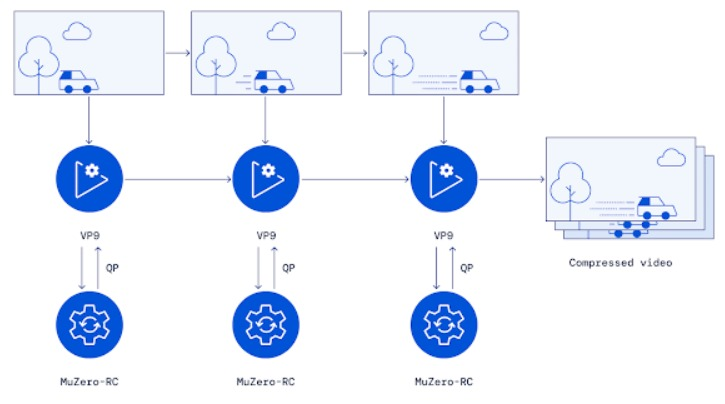
\includegraphics[width=0.4\textwidth]{sections/8Future Directions/MuZeroRC.jpg}

    \caption{MuZero Rate-Controller (MuZero-RC) optimizating the encoding process in video streaming.}
\end{figure}
\subsection*{AlphaFold}
AlphaFold is a model developed by DeepMind that addresses one of the
challenging problems in biology, which is predicting the three-dimensional
structures of proteins from their amino acid sequences. AlphaFold employs
advanced deep learning techniques, prominently featuring reinforcement
learning, to enhance its predictive capabilities.The model operates on a
feedback loop where it generates predictions about protein structures and
receives rewards based on the accuracy of these predictions compared to
experimentally determined structures. This process allows AlphaFold to
iteratively refine its models, optimizing them to better reflect the
complexities of protein folding dynamics. The architecture of AlphaFold
includes deep neural networks that analyze both the sequential and spatial
relationships between amino acids, enabling it to capture intricate patterns
for protein conformation. By training on extensive datasets of known protein
structures, AlphaFold has achieved unprecedented accuracy, often rivaling
experimental methods such as X-ray crystallography and cryo-electron
microscopy\cite{FD2}.\\\\ As shown form the previous models, how the employment
of reinforcementl learning changed starting from making AI systems which play
atari and strategy-based games, reaching to help in human biology and create
protein structures, the enployment of reinforcement learning in games still has
a long journey to be developed which helps in both real life and gaming. Google
DeepMind is still working on other models which are able to be implemented in
real life applications. They also developed models which use the multi-agent
models in games, like AlphaStar, which is a model to play StarCraft II; but
still didn't apply them in real life applications, which is a good future
direction to be developed.